\backmatter
%Formato de página sin header ni raya arriba
\renewcommand\headrulewidth{0pt}
\pagestyle{empty}
  \fancyhf{}
\fancypagestyle{plain}{}
\fancypagestyle{fancy}{}
\printindex{}

\begin{center}
%{\Huge A BOOK}
Cómo usar Google Earth Engine y no fallar en el intento, editado por el Centro de Investigaciones en Geografía Ambiental y el Instituto de Investigación de Recursos Biológicos Alexander von Humboldt se publicó el 20 de agosto de 2022. Para su formación se utilizaron las tipografías Latin Modern Roman y Computer Modern en 12, 15, 17 y 21 pt. El cuidado de la edición estuvo al cuidado de Jonathan Vidal Solórzano Villegas, Gabriel Alejandro Perilla Suárez, Mónica Braun y Jorge Andrés Trinidad González. El diseño editorial estuvo a cargo de Jonathan Vidal Solórzano Villegas y Laura Perilla Suárez.
%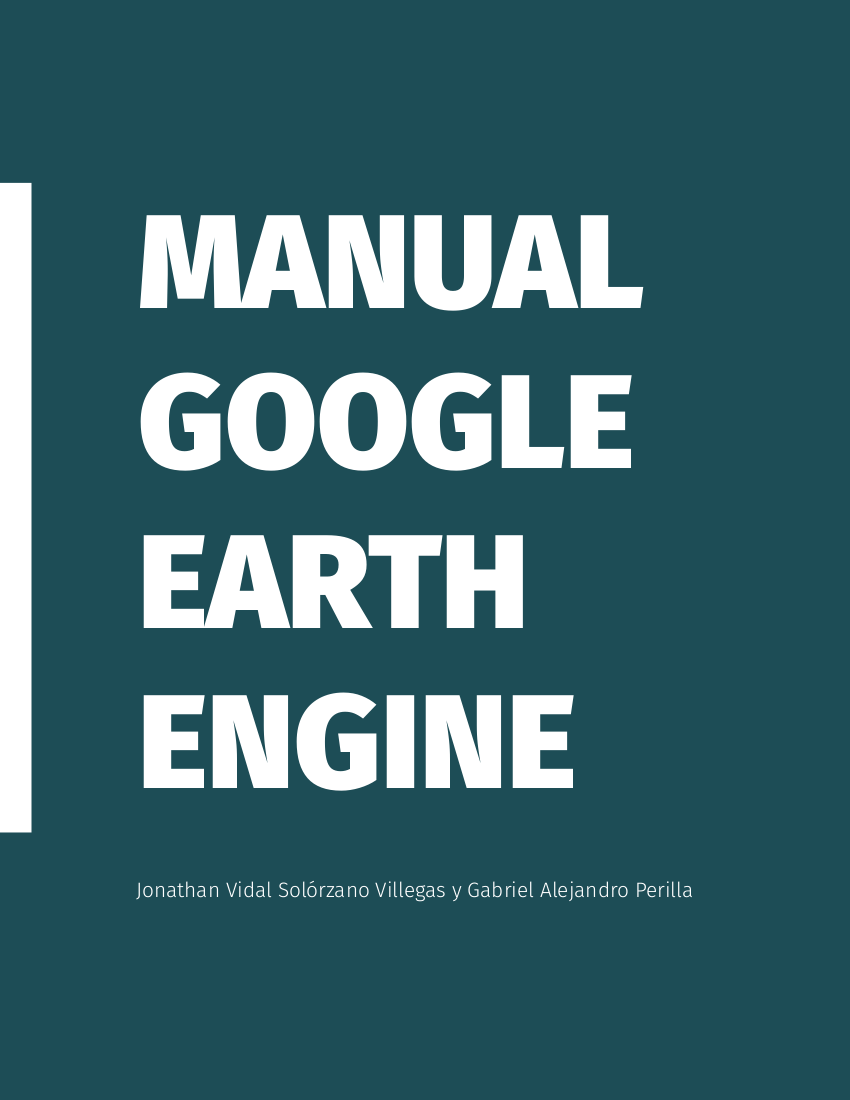
\includegraphics{Img/Portada.png}
%{\huge by Jonathan Vidal Solórzano Villegas y Alejandro Perilla Suárez}
\end{center}

\newpage
%\begin{center}
%  \begin{overpic}[height=1\textheight]{Img/ContraLogo.png}
%      \put(26,75){}
%  \end{overpic}
%{\Huge A BOOK}
\begin{center}
\includepdf[pagecommand={
  \begin{tikzpicture}[remember picture, overlay]
  \node[text height=15cm, text width=15cm, align=justify] at (0, 1) 
  {\textcolor{white}{\textbf{Google Earth Engine es una herramienta enfocada en facilitar el procesamiento de grandes volúmenes de información geoespacial. Por ello, ha permitido realizar análisis previamente imposibles de ejecutar en una computadora personal y acortar enormemente el tiempo de procesamiento requerido para realizar diferentes tipos de análisis. Este libro pretende fomentar el uso de esta poderosa herramienta entre usuarios hispanoparlantes y brindar una traducción al español de los principales tipos de objetos y métodos de esta plataforma. Este manual será de utilidad tanto para personas sin conocimiento de Google Earth Engine hasta aquellas con un nivel intermedio de uso, ya que aborda desde aspectos fundamentales hasta algunos consejos. También, ofrece ejemplos, códigos comentados, guías ilustradas, descripciones de la lógica de programación, detalles del funcionamiento interno, identificación de los errores más comunes y sus soluciones, y enlaces de utilidad que ayudarán al lector a aprender a utilizar Google Earth Engine o mejorar en sus capacidades de uso. Se recomienda enérgicamente que la lectura de este manual se haga en paralelo a la exploración de la plataforma y ejecutando todos los ejercicios. Finalmente, se espera que este libro permita aumentar el uso de Google Earth Engine y promover su uso para el desarrollo de diferentes tipos de investigaciones y aplicaciones.}}};
  \end{tikzpicture}}]{Img/ContraLogo.pdf}
%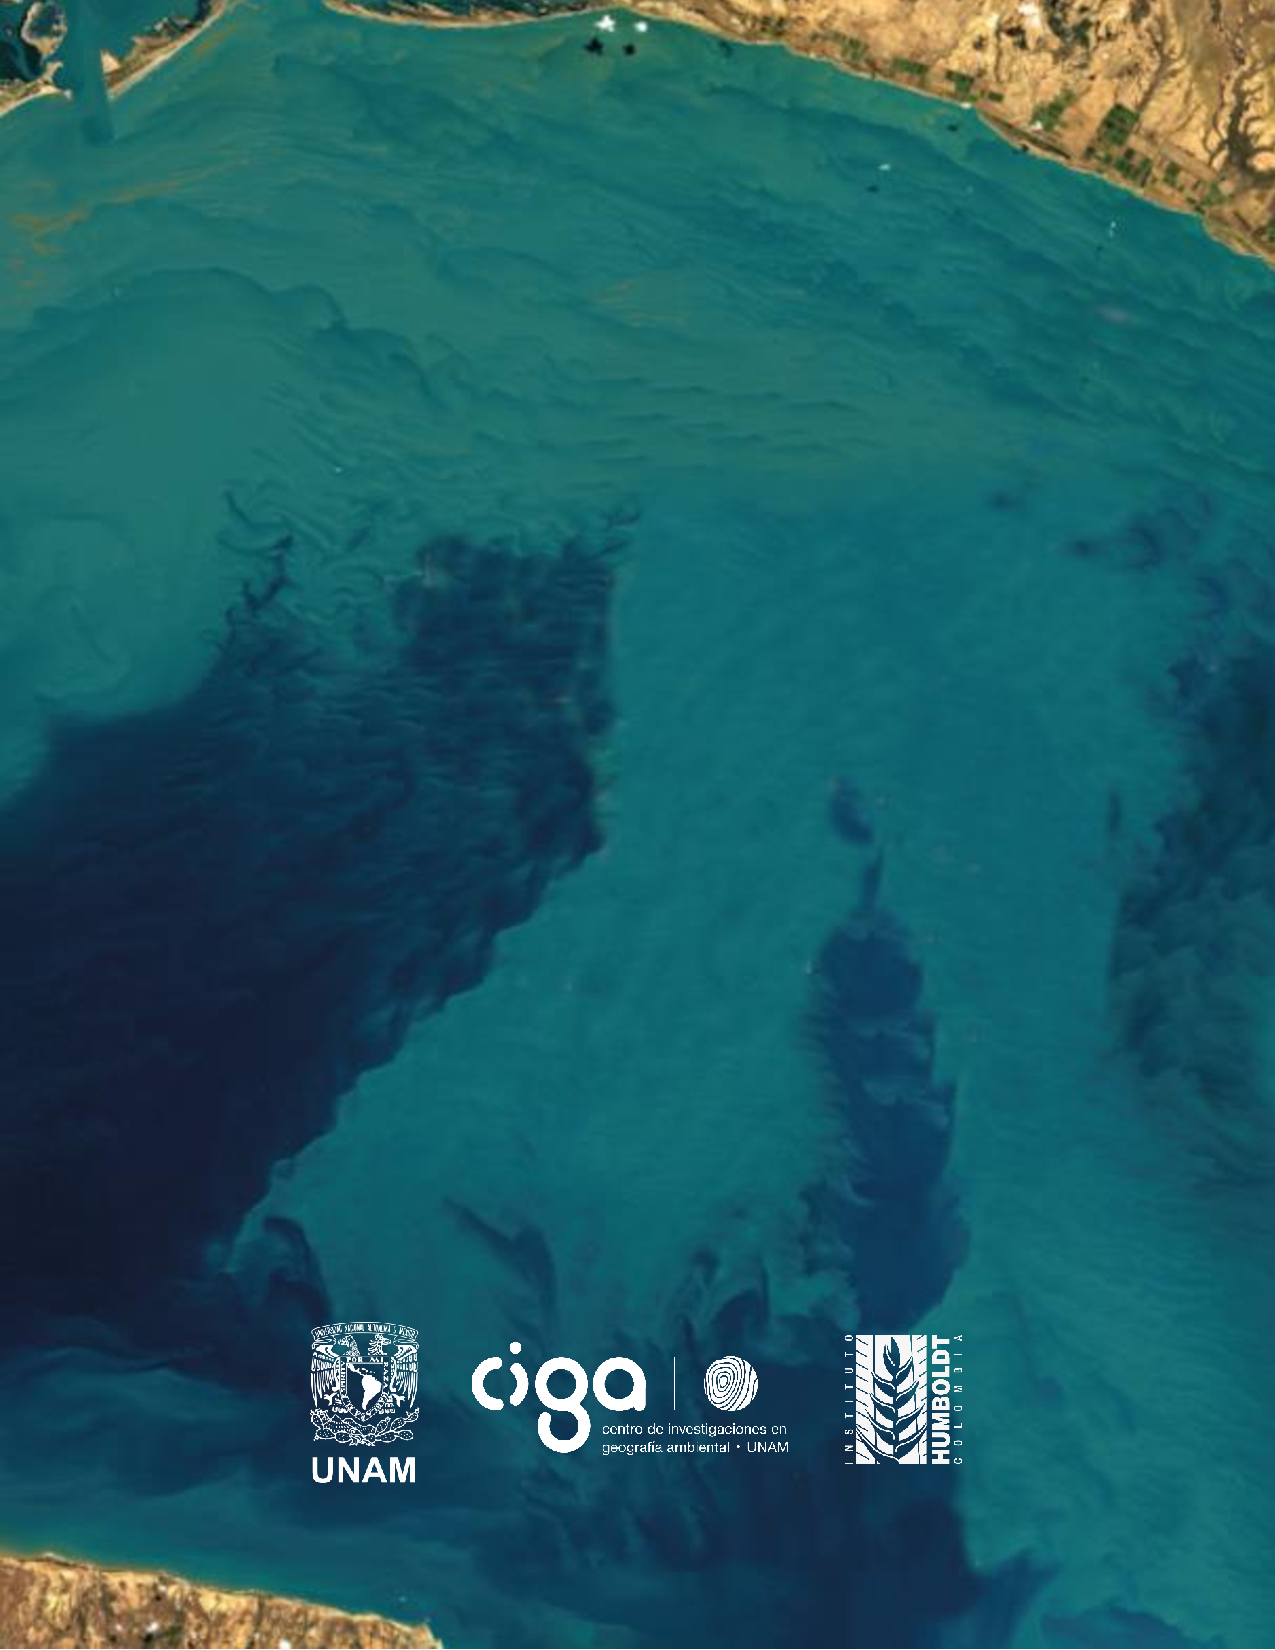
\includepdf{Img/ContraLogo.pdf}
%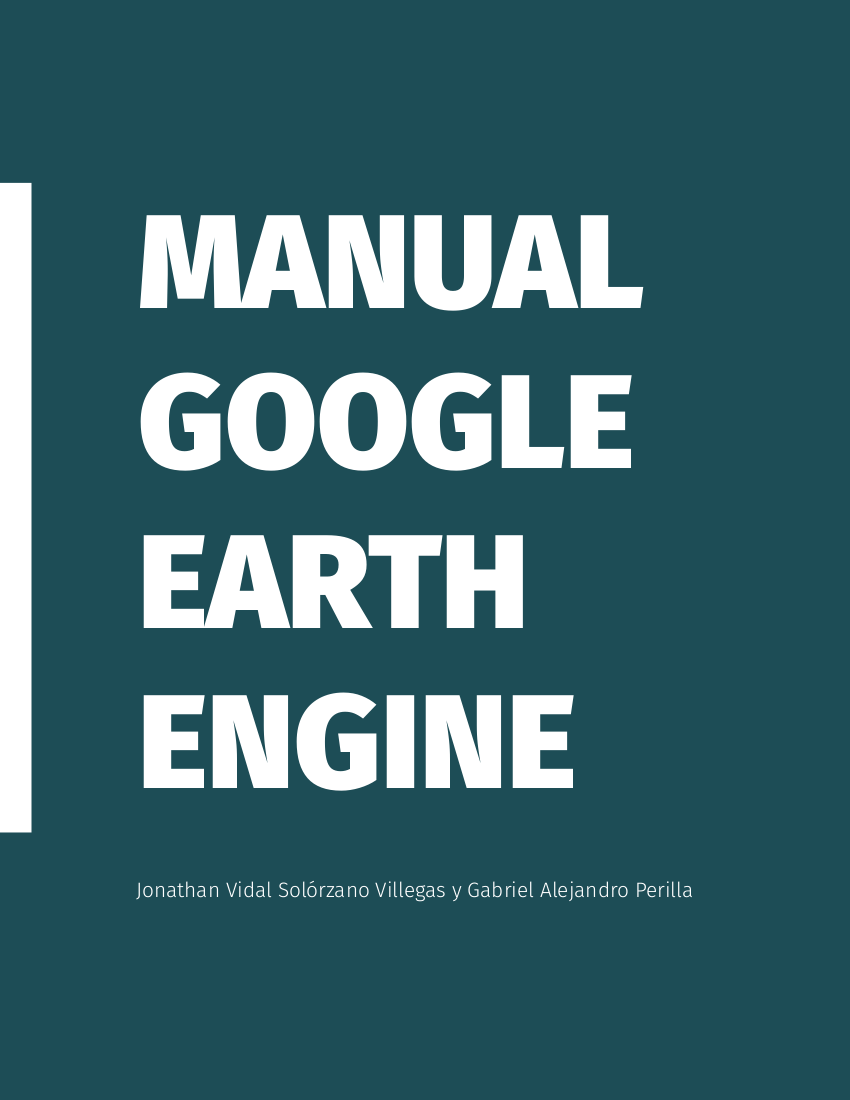
\includegraphics{Img/Portada.png}
%\large{Google Earth Engine es una herramienta enfocada en facilitar el procesamiento de grandes volúmenes de información geoespacial. Por ello, ha permitido realizar análisis previamente imposibles de ejecutar en una computadora personal y acortar enormemente el tiempo de procesamiento requerido para realizar diferentes tipos de análisis. Este libro pretende fomentar el uso de esta poderosa herramienta entre usuarios hispanoparlantes y brindar una traducción al español de los principales tipos de objetos y métodos de esta plataforma. Este manual será de utilidad tanto para personas sin conocimiento de Google Earth Engine hasta aquellas con un nivel intermedio de uso, ya que aborda desde aspectos fundamentales hasta algunos consejos. También, ofrece ejemplos, códigos comentados, guías ilustradas, descripciones de la lógica de programación, detalles del funcionamiento interno, identificación de los errores más comunes y sus soluciones, y enlaces de utilidad que ayudarán al lector a aprender a utilizar Google Earth Engine o mejorar en sus capacidades de uso. Se recomienda enérgicamente que la lectura de este manual se haga en paralelo a la exploración de la plataforma y ejecutando todos los ejercicios. Finalmente, se espera que este libro permita aumentar el uso de Google Earth Engine y promover su uso para el desarrollo de diferentes tipos de investigaciones y aplicaciones.}
\end{center}
